%-------------------------------------------------------------------
\section{Automated Problem Generation} \label{sec:ch5:algorithm}

With the discussion of the general problem class for \lqdo{} in Sec.~\ref{sec:ch5:lqdo} and \dt{} methods in Sec.~\ref{sec:ch5:formulation}, we can now describe the automated problem generation procedure (\apgp) for a variety of \dt{} methods used to create a \qp{} approximation.
Unlike general NLDO, all elements of the approximated \lqdo{} problem are associated with constant matrices in the \qp{}, so there is no need for finite-differencing or automatic differentiation to compute the Hessian or Jacobian \cite{Rao2010a}.
The matrices in the \qp{} problem tend to be large sparse matrices.
A sparse matrix is one in which when many of the elements are zero \cite{Betts2010a}.
In particular, the solution methods exhibit some form of a banded sparsity (and some localized dense blocks).
From the given formulas, it is straightforward to a determine the nonzero elements.
This motivates the sequence-based approach used to generate the triples (row locations, column locations, and values) that define a sparse matrix.

\subsection{Structure-Based Problem Definition}

The first piece of the \apgp{} is a natural description framework that describes \lqdo{} problems.
Here we use three different structure arrays to represent different problem elements, and they are outlined in a \textsc{c}-like notation in Fig.~\ref{fig:struct}. 
These structures are an easy-to-use interface between the user and the \apgp.

% structure

\begin{figure}%
\centering

\begin{subfigure}{0.3\textwidth}
\centering
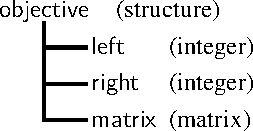
\includegraphics[scale=0.8]{../ch5/figures/objective}
\caption{Objective structure.}
\label{fig:struct:objective}
\end{subfigure}%
\begin{subfigure}{0.3\textwidth}
\centering
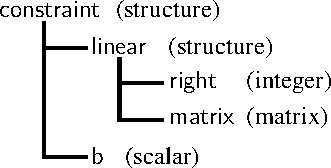
\includegraphics[scale=0.8]{../ch5/figures/constraint}
\caption{Constraint structure.}
\label{fig:struct:constraint}
\end{subfigure}%
\begin{subfigure}{0.3\textwidth}
\centering
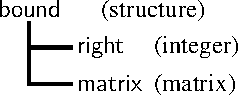
\includegraphics[scale=0.8]{../ch5/figures/bound}
\caption{Bound structure.}
\label{fig:struct:bound}
\end{subfigure}%

\caption{Structure definitions.}
\label{fig:struct}
\end{figure}

First, the structure definition in Fig.~\ref{fig:struct:objective} captures all of the objective terms outlined in Eqns.~(\ref{eq:ch5:QOFLagrange})--(\ref{eq:ch5:QOFMayer}).
The $\xvar{objective}$ structure is either $\mathcal{L}$ and $\mathcal{M}$ to account for Lagrange and Mayer terms, respectively.
Each entry in the structure is another term in the objective function.
The fields $\xvar{left}$ and $\xvar{right}$ can take on an integer value between $0$ and $5$, where $0$ indicates a singleton dimension (useful for linear and constant terms) and the remaining values correspond to the index of the expanded set of optimization variables introduced in Eqn.~(\ref{eq:ch5:varindices}).
Finally, $\xvar{matrix}$ is the potentially time-varying matrix of the appropriate size.
To illustrate this notation, consider the following LQ objective function: $\int_{t_0}^{t_f} \left[\sin(t) u_1^2(t) + \xi_2(t_0) \xi_1(t) \right] dt + \xi_1(t_f) -2 \xi_2(t_f)$.
The objective function can then be represented by the following\footnote{This example assumes $n_{\xi}=2$, $n_u=1$.}:%
\allowdisplaybreaks[1]%
\begin{subequations}%
\begin{align}
\int_{t_0}^{t_f}\sin(t) u_1^2(t)dt \ \Longleftrightarrow& \ \mathcal{L}\xind{1}.\xvar{left} = 1, \ \ \mathcal{L}\xind{1}.\xvar{right} = 1, \ \ \mathcal{L}\xind{1}.\xvar{matrix} = \sin(t) \\
% 
\int_{t_0}^{t_f}  \xi_2(t_0) \xi_1(t) dt \ \Longleftrightarrow& \ \mathcal{L}\xind{2}.\xvar{left} = 4, \ \ \mathcal{L}\xind{2}.\xvar{right} = 2, \ \ \mathcal{L}\xind{2}.\xvar{matrix} = \begin{bmatrix} 0 & 0 \\ 1 & 0 \end{bmatrix} \\
% 
\xi_1(t_f) -2 \xi_2(t_f) \ \Longleftrightarrow& \ \mathcal{M}\xind{1}.\xvar{left} = 0, \ \ \mathcal{M}\xind{1}.\xvar{right} = 5, \ \ \mathcal{M}\xind{1}.\xvar{matrix} = \begin{bmatrix} 1 \\ -2 \end{bmatrix}
\end{align}
\end{subequations}%
\allowdisplaybreaks[0]%

We now move onto the representation of the additional linear constraints in Eqns.~(\ref{eq:ch5:hqp})--(\ref{eq:ch5:gqp}).
The $\xvar{constraint}$ structure is either $\gls{Ycal}$ or $\gls{Zcal}$ to account for equality and inequality terms, respectively.
The field $\xvar{linear}$ can have multiple values to represent the summation needed for certain constraints.
The fields $\xvar{right}$ and $\xvar{matrix}$ are analogous to their use in the objective function terms.
The value for $\xvar{b}$ is the potentially time-varying function.
To illustrate this notation, consider the following linear constraints: $\xi_2(t_f) = 1$, $\xi_1(t) - 2 \xi_2(t) \leq 0$, and $u_1(t) - p_1 \leq \sin(t)$.
These linear constraints can then be represented by the following\footnote{This example assumes $n_{\xi}=2$, $n_u=1$, $n_p=1$.}:%
\allowdisplaybreaks[1]%
\begin{subequations}%
\small
\begin{align}
\xi_2(t_f) = 1 \ \Longleftrightarrow 
&\begin{cases}
\mathcal{Y}\xind{1}.\xvar{linear}\xind{1}.\xvar{right} = 5, \ \ \mathcal{Y}\xind{1}.\xvar{linear}\xind{1}.\xvar{matrix} = \begin{bmatrix} 0 \\ 1 \end{bmatrix}  \\
 \mathcal{Y}\xind{1}.\xvar{b} = 1 
\end{cases} \\
%
%
\xi_1(t) - 2 \xi_2(t) \leq 0 \ \Longleftrightarrow 
&\begin{cases}
\mathcal{Z}\xind{1}.\xvar{linear}\xind{1}.\xvar{right} = 2, \mathcal{Z}\xind{1}.\xvar{linear}\xind{1}.\xvar{matrix} = \begin{bmatrix} 1 \\ -2 \end{bmatrix} \\
\mathcal{Z}\xind{1}.\xvar{b} = 0 
\end{cases} \\
%
%
u_1(t) - p_1 \leq \sin(t) \ \Longleftrightarrow 
&\begin{cases}
\mathcal{Z}\xind{2}.\xvar{linear}\xind{1}.\xvar{right} = 1, \ \ \mathcal{Z}\xind{2}.\xvar{linear}\xind{1}.\xvar{matrix} = 1 \\
\mathcal{Z}\xind{2}.\xvar{linear}\xind{2}.\xvar{right} = 3, \ \ \mathcal{Z}\xind{2}.\xvar{linear}\xind{2}.\xvar{matrix} = -1 \\
\mathcal{Z}\xind{2}.\xvar{b} = \sin(t)
\end{cases}
\end{align}
\end{subequations}%
\allowdisplaybreaks[0]%

The $\xvar{bound}$ structure is used to represent additional linear constraints that can be written as simple upper and lower bounds as in Eqn.~(\ref{eq:ch5:simplebounds}).
Then the structure is either $\gls{UBcal}$ or $\gls{LBcal}$ to account for upper and lower terms, respectively.
The fields $\xvar{right}$ and $\xvar{matrix}$ are used analogously as the previous structures, with the exception that the values of $\xvar{matrix}$ can be $\pm \infty$ to indicate no bounds when appropriate.
To illustrate this notation, consider the following simple bounds: $u_1(t) \geq \sin(t)$ and $\xi_2(t) \leq \pi$.
Then these bounds can be represented by the following\footnote{This example assumes $n_{\xi}=2$, $n_u=1$.}:%
\begin{subequations}%
\begin{align}
u_1(t) \geq \sin(t) \quad \Longleftrightarrow& \quad \mathcal{LB}\xvar{\myind{1}.right} = 1, \quad \mathcal{LB}\xvar{\myind{1}.matrix} = \sin(t) \\
\xi_2(t) \leq \pi \quad \Longleftrightarrow& \quad \mathcal{UB}\xvar{\myind{1}.right} = 1, \quad \mathcal{UB}\xvar{\myind{1}.matrix} = \begin{bmatrix} \infty \\ \pi \end{bmatrix}
\end{align}
\end{subequations}%

%------------------------------------------------------------
\subsection{Procedure Overview}

A schematic overview of the \apgp{} is shown in Fig.~\ref{fig:overview}.
The user provides the problem structure using the notation defined in the previous section along with their choices for the mesh, quadrature, and defect constraints (these options are colored \textcolor{red}{red}).
These options are related to the acronyms used in Sec.~\ref{sec:ch5:formulation}.
We note that in addition to ED, LGL, and CGL mesh schemes, a user-defined mesh is also possible.
First, the mesh is generated and a number of initialization tasks are performed.
Next, the algorithms in the dashed box are presented in a modular format as the problem elements in \lqdo{} are separate, and are utilized only when necessary as they approximate specific problem elements.
Once all elements of the problem are approximated, the set of matrices that define the \qp{} are passed to an appropriate \qp{} solver to find the solution.

\tikzexternalexportnextfalse
\begin{figure}
\centering

\tikzstyle{block} = [rectangle, draw, fill=white, text centered, minimum height=2em, text width=9.5em]
\tikzstyle{block2} = [rectangle, draw, fill=white, text centered, minimum height=2em, text width=11.4em]
\tikzstyle{block3} = [rectangle, draw=red, text=red, fill=white, text centered, minimum height=2em, text width=5.5em]
\tikzstyle{block4} = [rectangle, draw=red, text=red, fill=white, text centered, minimum height=2em, text width=5.5em]
\tikzstyle{line} = [draw, -latex']
\tikzstyle{cloud} = [draw, ellipse,fill=white, node distance=3cm,
    minimum height=2em]

% \tikzset{every loop/.style={min distance=10mm,in=-185,out=-175,looseness=0}}

\tikzsetnextfilename{overview}
\resizebox{5in}{!}{%
\begin{tikzpicture}[
    pre/.style={>=latex',semithick},
    post/.style={>=latex,shorten >=1pt,>=latex',semithick,line width=1pt},
    mydouble/.style={<->, >=latex,shorten >=1pt,>=latex',semithick,line width=1pt},
    node distance = 3cm, auto
    ]
     
    \tikzset{
  manual input/.style={
    shape=trapezium,
    draw,
    shape border rotate=90,
    trapezium left angle=90,
    trapezium right angle=85}}

    % Place nodes
    
    % \node [] (solve) {solve};
    
    % \node [block, below=0.8cm of solve] (create) {create};
    \node [cloud] (create) {Problem structure};
    
    %
	\node [block, below=0.8cm of create] (initialize) {Initialize};
    
    \node [block2, right=0.8cm of initialize] (createT) {Create $\bm{t}$};
    
    \node [block3, manual input, above right=-0.4cm and 1.4cm of createT] (createTmethods) {\scriptsize ED, LGL, CGL, USER};
    
    %
	\node [block, below=0.8cm of initialize] (createH) {Hessian term \\ (see Alg.~\ref{alg:ch5:hessian})};
        
    %
	\node [block, below=0.8cm of createH] (createF) {Gradient term \\ ($\sim$ to Alg.~\ref{alg:ch5:hessian})};   
   
    %
	\node [block, below=0.8cm of createF] (createC) {Constant term \\ ($\sim$ to Alg.~\ref{alg:ch5:hessian})};  
    
	\node [block2, above right=-0.0cm and 0.8cm of createF] (Lbig) {$\mathcal{L}^{QP}$ terms (see Alg.~\ref{alg:ch5:Lterms})};
    
    \node [block3, manual input, above right=-0.4cm and 1.4cm of Lbig] (Lsmallmethods) {\scriptsize CEF, CTR, CQHS, G, CC};
    
	\node [block2, below right=-0.0cm and 0.8cm of createF] (Mbig) {$\mathcal{M}^{QP}$ terms (see Alg.~\ref{alg:ch5:Mterms})};
    

    %
	\node [block, below=0.8cm of createC] (createdefects) {Defect constraints \\ (see Algs.~\ref{alg:ch5:SSdefects}--\ref{alg:ch5:PSdefects})};
    
    \node [block4, manual input, right=3cm of createdefects] (Defectmethods) {\scriptsize ZOH, EF, TR, HS, RK4, PS};
    
    %
	\node [block, below=0.8cm of createdefects] (createYZ1) {Add. eq. constraints \\ (see Alg.~\ref{alg:ch5:constraints})};
    
    % \node [block2, above right=-0.43cm and 0.8cm of createYZ1] (path1) {$\bm{C}$ terms (see Alg.~\ref{})};
    
	% \node [block2, below right=-0.43cm and 0.8cm of createYZ1] (boundary1) {$\bm{\phi}$ terms (see Alg.~\ref{})};
    
    \node [block2, below right=-0.55cm and 0.8cm of createYZ1] (path) {$\bm{C}$ terms (see Alg.~\ref{alg:ch5:path})};
    
    %
	\node [block, below=0.8cm of createYZ1] (createYZ2) {Inequality constraints \\ (see Alg.~\ref{alg:ch5:constraints})};
    
    % \node [block2, above right=-0.43cm and 0.8cm of createYZ2] (path2) {$\bm{C}$ terms (see Alg.~\ref{})};
    
	% \node [block2, below right=-0.43cm and 0.8cm of createYZ2] (boundary2) {$\bm{\phi}$ terms (see Alg.~\ref{})};
       
	\node [block2, above right=-0.55cm and 0.8cm of createYZ2] (boundary) {$\bm{\phi}$ terms (see Alg.~\ref{alg:ch5:boundary})};
       
    \node [block, below=0.8cm of createYZ2] (createBnds) {Simple bounds \\ ($\sim$ to Alg.~\ref{alg:ch5:constraints})};
    
    \node [cloud, below=0.8cm of createBnds] (qpsolver) {To QP solver};
    
    \node [above right=-1.3cm and 1.4cm of qpsolver] (qp) {\begin{minipage}{0.3\textwidth}\textcolor{black!70}{
\begin{align*}
\min_{\mathbf{X}} \qquad& \frac{1}{2}\mathbf{X}\tran \mathbf{H} \mathbf{X} + \mathbf{F}\tran \mathbf{X} + c \\
\text{subject to:} \qquad& \begin{bmatrix} \mathbf{A}_{e1} \\ \mathbf{A}_{e2} \end{bmatrix}\mathbf{X} = \begin{bmatrix} \mathbf{B}_{e1} \\ \mathbf{B}_{e2} \end{bmatrix} \\
& \mathbf{A}_{i}\mathbf{X} \leq \mathbf{B}_{i} \\
& \myunderbar{\mathbf{X}} \leq \mathbf{X} \leq \myoverbar{\mathbf{X}} 
\end{align*}}
\end{minipage}};
    
    % outputs
	\node [left=0.8cm of createH] (outputH) {$\mathbf{H}$};
    
    \node [left=0.8cm of createF] (outputF) {$\mathbf{F}$};
    
    \node [left=0.8cm of createC] (outputC) {$c$};
    
    \node [left=0.8cm of createdefects] (outputdefects) {$\mathbf{A}_{e1}, \mathbf{B}_{e1}$};
    
    \node [left=0.8cm of createYZ1] (outputYZ1) {$\mathbf{A}_{e2}, \mathbf{B}_{e2}$};
    
    \node [left=0.8cm of createYZ2] (outputYZ2) {$\mathbf{A}_{i}, \mathbf{B}_{i}$};
    
    \node [left=0.8cm of createBnds] (outputBnds) {$\myunderbar{\mathbf{X}}$, $\myoverbar{\mathbf{X}}$};
    
    % boxes
	\node [dashed,  draw=black, minimum width=12em, minimum height=13.75cm, above=-13.5cm of createH] (method) {};
    
    % Draw edges
    \path [post, line] (createH) -- (outputH);
    \path [post, line] (createF) -- (outputF);
    \path [post, line] (createC) -- (outputC);
    \path [post, line] (createdefects) -- (outputdefects);
    \path [post, line] (createYZ1) -- (outputYZ1);
    \path [post, line] (createYZ2) -- (outputYZ2);
    \path [post, line] (createBnds) -- (outputBnds);
    
    % \path [post, line] (initialize) -- (createT);
    \path [mydouble, draw] (createT) -- (initialize);
    
    % \path [post, line] (createH.east) -- (Lbig.170);
    \path [mydouble, draw] (Lbig.175) -- (createH.east);
    
    % \path [post, line] (createH.east) -- (Mbig.170);
    \path [mydouble, draw] (Mbig.175) -- (createH.east);
    
    % \path [post, line] (createF.east) -- (Lbig.west);
    \path [mydouble, draw] (Lbig.west) -- (createF.east);
    
    % \path [post, line] (createF.east) -- (Mbig.west);
    \path [mydouble, draw] (Mbig.west) -- (createF.east);
    
    % \path [post, line] (createC.east) -- (Lbig.190);
    \path [mydouble, draw] (Lbig.185) -- (createC.east);
    
    % \path [post, line] (createC.east) -- (Mbig.190);
    \path [mydouble, draw] (Mbig.185) -- (createC.east);
        
    % \path [post, line] (createYZ1.east) -- (boundary.175);
    \path [mydouble, draw] (boundary.west) -- (createYZ1.east);
    
    % \path [post, line] (createYZ2.east) -- (boundary.185);
    \path [mydouble, draw] (boundary.west) -- (createYZ2.east);
    
    % \path [post, <->, line] (createYZ1.east) -- (path.175);
    \path [mydouble, draw] (path.west) -- (createYZ1.east);
    
    % \path [post, <->, line] (createYZ2.east) -- (path.185);
    \path [mydouble, draw] (path.west) -- (createYZ2.east);

   % \path [post, line] (Lbigmethods) -- (Lbig);
    
	\path [post, line] (Lsmallmethods.west) -- (Lbig.east);

    % \path [post, line] (Lsmallmethods.west) -- (Lsmall.east);
    
    % \path [post, line] (Lsmallmethods.west) -- (Lconstant.east);
    
    % \path [post, line] (Lconstantmethods) -- (Lconstant);
    
    \path [post, line] (Defectmethods.west) -- (createdefects.east);
    
    \path [post, line] (createTmethods.west) -- (createT.east);
    

\draw [decorate,decoration={brace,amplitude=10pt},xshift=-4pt,yshift=0pt]
(-3.3,-7.7) -- (-3.3,-3.2) node [black,midway,xshift=-0.3cm] 
{\footnotesize \rotatebox{90}{Objective function}};

\draw [decorate,decoration={brace,amplitude=10pt},xshift=-4pt,yshift=0pt]
(-4.4,-15.7) -- (-4.4,-9.1) node [black,midway,xshift=-0.3cm] 
{\footnotesize \rotatebox{90}{Constraints}};

% straight down
    \path [post, line] (create) -- (initialize);
    \path [post, line] (initialize.south) -- (method.north);
    \path [post, line] (method.south) -- (qpsolver.north);

\end{tikzpicture}
}
% \vspace{-0.3in}
\caption{Overview of the automated problem generation procedure.}\label{fig:overview}

\end{figure}

%------------------------------------------------------------
\subsection{Algorithms}

Here we briefly describe the algorithms with the full pseudocodes in Sec.~\ref{sec:app3:algorithms}.
The first algorithm outlines two functions used to get index sequence of the variable's location in both the continuous and discrete problems.
The function \textsc{GetContIndex} takes an integer between $0$ and $5$, used to denote a set of optimization variables in $\tilde{\bm{x}}$, and returns the sequence defining all the locations of that particular class of optimization variables in Eqn.~(\ref{eq:ch5:x:cont}).
The second function, \textsc{findQPindex}, requires three inputs: 1) \xvar{x} is the specific number of the optimization variable that is selected, 2) \xvar{xtype} is the same optimization variable classification as before, and 3) \xvar{idx} are the necessary indices to return.
For example, if $n_u = 2$, $n_{\xi} = 3$, and $n_{p} = 1$, then $\xvar{x}$ could be valued from $0$ to $6$ since there are $6$ total optimization variables.
Continuing with this example, if $\xvar{x} = 4$, $\xvar{xtype} = 2$, and $\xvar{idx} = 1 \text{ to } N_t$, then we are requesting the indices of the discretization of $\xi_2(t)$, i.e.,~$\mathbf{X}(\xvar{I}) = \xi_2(\bm{t})$.
Both of these functions will be useful when creating the objective function terms and additional linear constraints.

\subsubsection{Objective Function Terms} \label{sec:ch5:alg:objective}

There are three main algorithms are used to implement the five methods for approximating objective function terms in Sec.~\ref{sec:ch5:dt:objective}.
The Lagrange terms are approximated by quadrature in Alg.~\ref{alg:ch5:Lterms}.
The input is a structure $\mathcal{L}$ of type \xvar{objective} and for each substructure, the relevant sequences are created.
Both the \textsc{GetContIndex} and \textsc{GetQPIndex} are used to generate the appropriate row and column locations in the Hessian.
While the CQHS method is shown specifically, the other quadrature schemes can readily be implemented with the same pseudocode with modifications to lines \ref{line:ch5:V}--\ref{line:ch5:Voff} pertaining to the values of the diagonal and off-diagonal entries.
To visualize the process being used in Alg.~\ref{alg:ch5:Lterms}, the sparsity pattern for different $\bm{L}_{ij}$ is shown in Fig.~\ref{fig:figsparsityHSS}.
Each concatenation of \xvar{I} on line~\ref{line:ch5:lqp_I} in the algorithm is the addition of a single diagonal in Fig.~\ref{fig:figsparsityHSS}b or column in Fig.~\ref{fig:figsparsityHSS}d.

Compact and efficient formulas for the quadrature methods are achieved by the creation of $\xvar{H}$ (and similar terms) and the use of the $\textsc{rshift}$ function.
Consider the CTR method: 
\begin{align}
\begin{matrix}
\xvar{H} & =[& \Delta_0 & \Delta_1 & \cdots & \Delta_{n_t-1} & 0 &]  \\
\text{\textsc{rshift}}(\xvar{H}) & =[&  0 & \Delta_0 & \cdots & \Delta_{n_t-2} & \Delta_{n_t-1} &] \\
\xvar{Q} & =[&  \xvar{A}(t_0) & \xvar{A}(t_1) & \cdots & \xvar{A}(t_{n_t-1}) & \xvar{A}(t_{n_t})  &] \\
\text{CTR} & =[&  \Delta_0 \xvar{A}(t_0) & (\Delta_0+\Delta_1) \xvar{A}(t_1) & \cdots & (\Delta_{n_t-2}+\Delta_{n_t-1}) \xvar{A}(t_{n_t-1}) & \Delta_{n_t-1} \xvar{A}(t_{n_t}) &]
\end{matrix} 
\end{align}

\noindent We see the formula $\left( \xvar{H} \oplus \text{\textsc{rshift}}(\xvar{H}) \right)  \odot \xvar{Q}/2$ produces the appropriate entries for the CTR method in Eqn.~(\ref{eq:ch5:CTR}).

% new paragraph
The sequences for the Mayer terms are created with Alg.~\ref{alg:ch5:Mterms}, which is similar to the algorithm for the Lagrange terms.
The approximation of Mayer terms is the same across the quadrature methods as previously mentioned.

% new paragraph
To create the sparse Hessian matrix, Alg.~\ref{alg:ch5:hessian} takes the sequences from both Algs.~\ref{alg:ch5:Lterms}--\ref{alg:ch5:Mterms}.
The creation of the gradient and constant terms in Eqn.~(\ref{eq:ch5:qpH}) requires some minor modifications to Alg.~\ref{alg:ch5:hessian} but requires no modifications of Algs.~\ref{alg:ch5:Lterms}--\ref{alg:ch5:Mterms}. 

%------------------------------------------------------------
\subsubsection{Defect Constraints}

The algorithms for creating the defect constraints are shown in Alg.~\ref{alg:ch5:SSdefects} (SS methods) and Alg.~\ref{alg:ch5:PSdefects} (PS methods).
We will first describe the approach used for the SS methods based on Eqns.~(\ref{eq:ch5:ssdefects})--(\ref{eq:ch5:ssdefectsZOH}).
All required defect constraints for a particular state are generated inside the for-loop on line~\ref{line:ch5:SSdefects_for}.
In order, the appropriate entries in the matrix $\mathbf{A}_{e1}$ are generated for the controls, states, and parameters based on their $\bm{\theta}$ term expressions (see Eqn.~(\ref{eq:ch5:ss})).
The sparsity pattern for this matrix is shown in Fig.~\ref{fig:figsparsityASS}.
The row and column locations are generated through the appropriate sequences based on the number of variables and node points.
The values of the matrix entries are computed with element-wise formulas, similar to the approach used in the objective function terms (see Sec.~\ref{sec:ch5:alg:objective}).
The indexing vector $\xvar{T}$ allows us to extract matrix values on different time grids shifted by one index which are present due to the shifting of $k$ and $k+1$ values in the formulas.
Using this approach, all time-varying functions are evaluated only once on a particular time grid.

% new paragraph
The \textsc{kron} function\cite{matlab-kron} used on line~\ref{line:ch5:SSdefects_kron} generates a matrix that efficiently implements $\bm{I}$ in the equations (see its usage on lines~\ref{line:ch5:SSdefects_V1}--\ref{line:ch5:SSdefects_V2}).
For the states and controls, values are calculated for the lower and upper diagonals in their respective blocks.
For the controls, the lower diagonal values ($\bm{\theta}_1$ terms) are computed on line~\ref{line:ch5:SSdefects_V3} and the upper diagonal ($\bm{\theta}_2$ terms) are computed on the following line.
These diagonals are visualized in Figs.~\ref{fig:figsparsityASS}c--d.
Once the row, columns, and values for each state's defect constraints are generated, they are combined into a single sparse matrix of size $n_{\xi} n_t \times n_{X}$.
The disturbance in Eqn.~(\ref{eq:ch5:ss}) is the only part of the dynamics that appears in the $\mathbf{B}_{e1}$ term.
It is created in a similar fashion as the parameters (except there is only a single column in the resulting matrix).
The algorithm presented specifically implements the TR method, but can be readily adapted to the other SS methods (the formulas for \xvar{V} would need to be updated).

% new paragraph
For PS methods (both with LGL or CGL nodes) in Alg.~\ref{alg:ch5:PSdefects}, there is one more defect constraint per state than for an equivalent SS method.
Overall, the procedure is very similar to the one for SS methods.
The indexing vector $\xvar{T}$ is not needed since the matrix values only require the derivative function values at a single point in time in each row of the defect constraint (see the sparsity pattern in Figs.~\ref{fig:figsparsityAPS}b--d).
Instead of \xvar{K}, a PS method requires the differentiation matrix $\bm{D}$ to be provided.
This matrix is appropriately copied and shifted so that it coincides with the defect constraint rows and columns for the current state (see line~\ref{line:ch5:D}).
This is visualized with the block dense matrices in Fig.~\ref{fig:figsparsityAPS}a.

%------------------------------------------------------------
\subsubsection{Additional Linear Constraints and Bounds} \label{sec:ch5:alg:lin:constraints}

Both the additional inequality and equality constraints are created using Alg.~\ref{alg:ch5:constraints} taking in a structure of type $\textsf{constraint}$.
For each substructure (i.e.,~for each different constraint), we need to determine if its type is either path or boundary.
There are two conditions such that a constraint can be considered a path constraint: 1) any of the variable types in \textsf{right} are controls or states; 2) any of the matrices are time-varying (e.g.,~$\bm{Z}_3(t)$ or $\hat{Z}(t)$).

% new paragraph
If it is determined that the constraint is a path constraint, then Alg.~\ref{alg:ch5:path} is utilized to create the sparse matrix sequences.
Otherwise, Alg.~\ref{alg:ch5:boundary} is utilized.
These two algorithms are quite similar, the primary difference being how many constraints are created ($N_t$ vs. one).
Both utilize \textsc{GetContIndex} and \textsc{GetQPIndex} in a similar fashion to the objective function terms in Sec.~\ref{sec:ch5:alg:objective}.
After all sequences are created and combined, the sparse matrix is generated.

% new paragraph
For simple bounds in Eqn.~(\ref{eq:ch5:simplebounds}), the \textsf{bound} structure type is used.
The same algorithms are applicable but the entries are initialized as either $-\infty$ or $\infty$ depending on if it is a lower or upper bound.
This ensures that unconstrained variables remain unconstrained.